\documentclass[11pt]{beamer}

%%% \mode must be on a line by its own, without comment or whitespace!
%%% \mode sets the mode to presentation. So if the mode is presentation the slides after are shown
%%% if the mode is not presentation (but article or handout) they are not shown
\mode<presentation>{}

\usetheme{Warsaw}
\usepackage[utf8]{inputenc}
\usepackage[english]{babel}
\usepackage{amsmath}
\usepackage{amsfonts}
\usepackage{amssymb}
\usepackage{graphicx}
\usepackage{xspace}

\author{Guus Bonnema}
\title{Final Presentation\\(XMas Designer)}
%\setbeamercovered{transparent} 
%\setbeamertemplate{navigation symbols}{} 
%\logo{} 
\institute{Open University\\team033\\Guus Bonnema, Stefan Versluys, Jeroen Kleijn} 
\date{May 20, 2015} 
\subject{ABI project XMas Designer} 

\begin{document}

\newcommand{\Noc}{\textsc{NoC}\xspace}
\newcommand{\qt}{\textsc{Qt}\xspace}
\newcommand{\qml}{\textsc{Qml}\xspace}

\begin{frame}
	\titlepage
\end{frame}

\begin{frame}{Who are we?}
	\begin{description}
		\item[Guus Bonnema]	Student Computer Science
							Dayjob: functional maintenance
		\item[Jeroen Kleijn] Student Computer Science
							 Dayjob: ...............
		\item[Stefan Versluys]	Student Computer Science
								Dayjob: C++ embedded programming
	\end{description}
\end{frame}

\begin{frame}{Assignment}
	\begin{columns}
		\begin{column}[t]{5cm}
		{\bf Customer needs}

		Create a {\it platform independent}, {\it maintainable} application that supports
		developing Network on Chip (\Noc) designs and supports adding verification tools
		to check the \Noc designs for cycles and deadlocks. The tool should {\it integrate well}
		with our existing C++ tools.
		
		Options are a rewrite
		of the current tool or a refactor.
		\end{column}
		\begin{column}[t]{5cm}
		{\bf Project intentions}		
		
		Using only multi-platform tools we aimed at creating a C++ tool for creating
		and maintaining \Noc networks.
		
		Refactor seemed improbable as best solution
		\end{column}
	\end{columns}
\end{frame}

\begin{frame}{Overview Process}
	\begin{columns}
		\begin{column}[t]{5cm}
			Process
			\begin{itemize}
				\item <1->Planning phase: DAD approach (Disciplined Agile Delivery)
				\item <1->Domain analyses
				\item <1->Iteration 0 Architecture
				\item <1->Iteration 1 Build procedures and first prototype
				\item <1->iteration 2, 3, 4, 5 software development
				\item <1->\textit{Final Demo}$\leftarrow$
				\item <1->\textbf{transition}
			\end{itemize}
		\end{column}
		\begin{column}[t]{5cm}
			Development factors
			\begin{itemize}
				\item <2->Time boxing
				\item <2->Early switch to \qt
				\item <2->UI design : \qml
				\item <2->Qml / xmas integration: fat interface
				\item <2->Reorg OU $\rightarrow$ Communication drop
			\end{itemize}
		\end{column}
	\end{columns}
\end{frame}

\begin{frame}{Contribution to research project}

	\begin{itemize}
		\item {\bf Research}
		\begin{itemize}
			\item support for papers to reason about verification tools of NoC
			\item support for developers and testers of verification tools
			\item support for marketing of research efforts at OU and Radboud university
		\end{itemize}
		\item {\bf Design}
		\begin{itemize}
			\item support for designs of NoC
		\end{itemize}
	\end{itemize}

\end{frame}

\begin{frame}{Example NoC}

\end{frame}

\begin{frame}{Demo XMAS Designer}
	Demo : how? Who will do it? how long? Prerecorded?
\end{frame}

\begin{frame}{Specification model Data Layer iteration 1}

	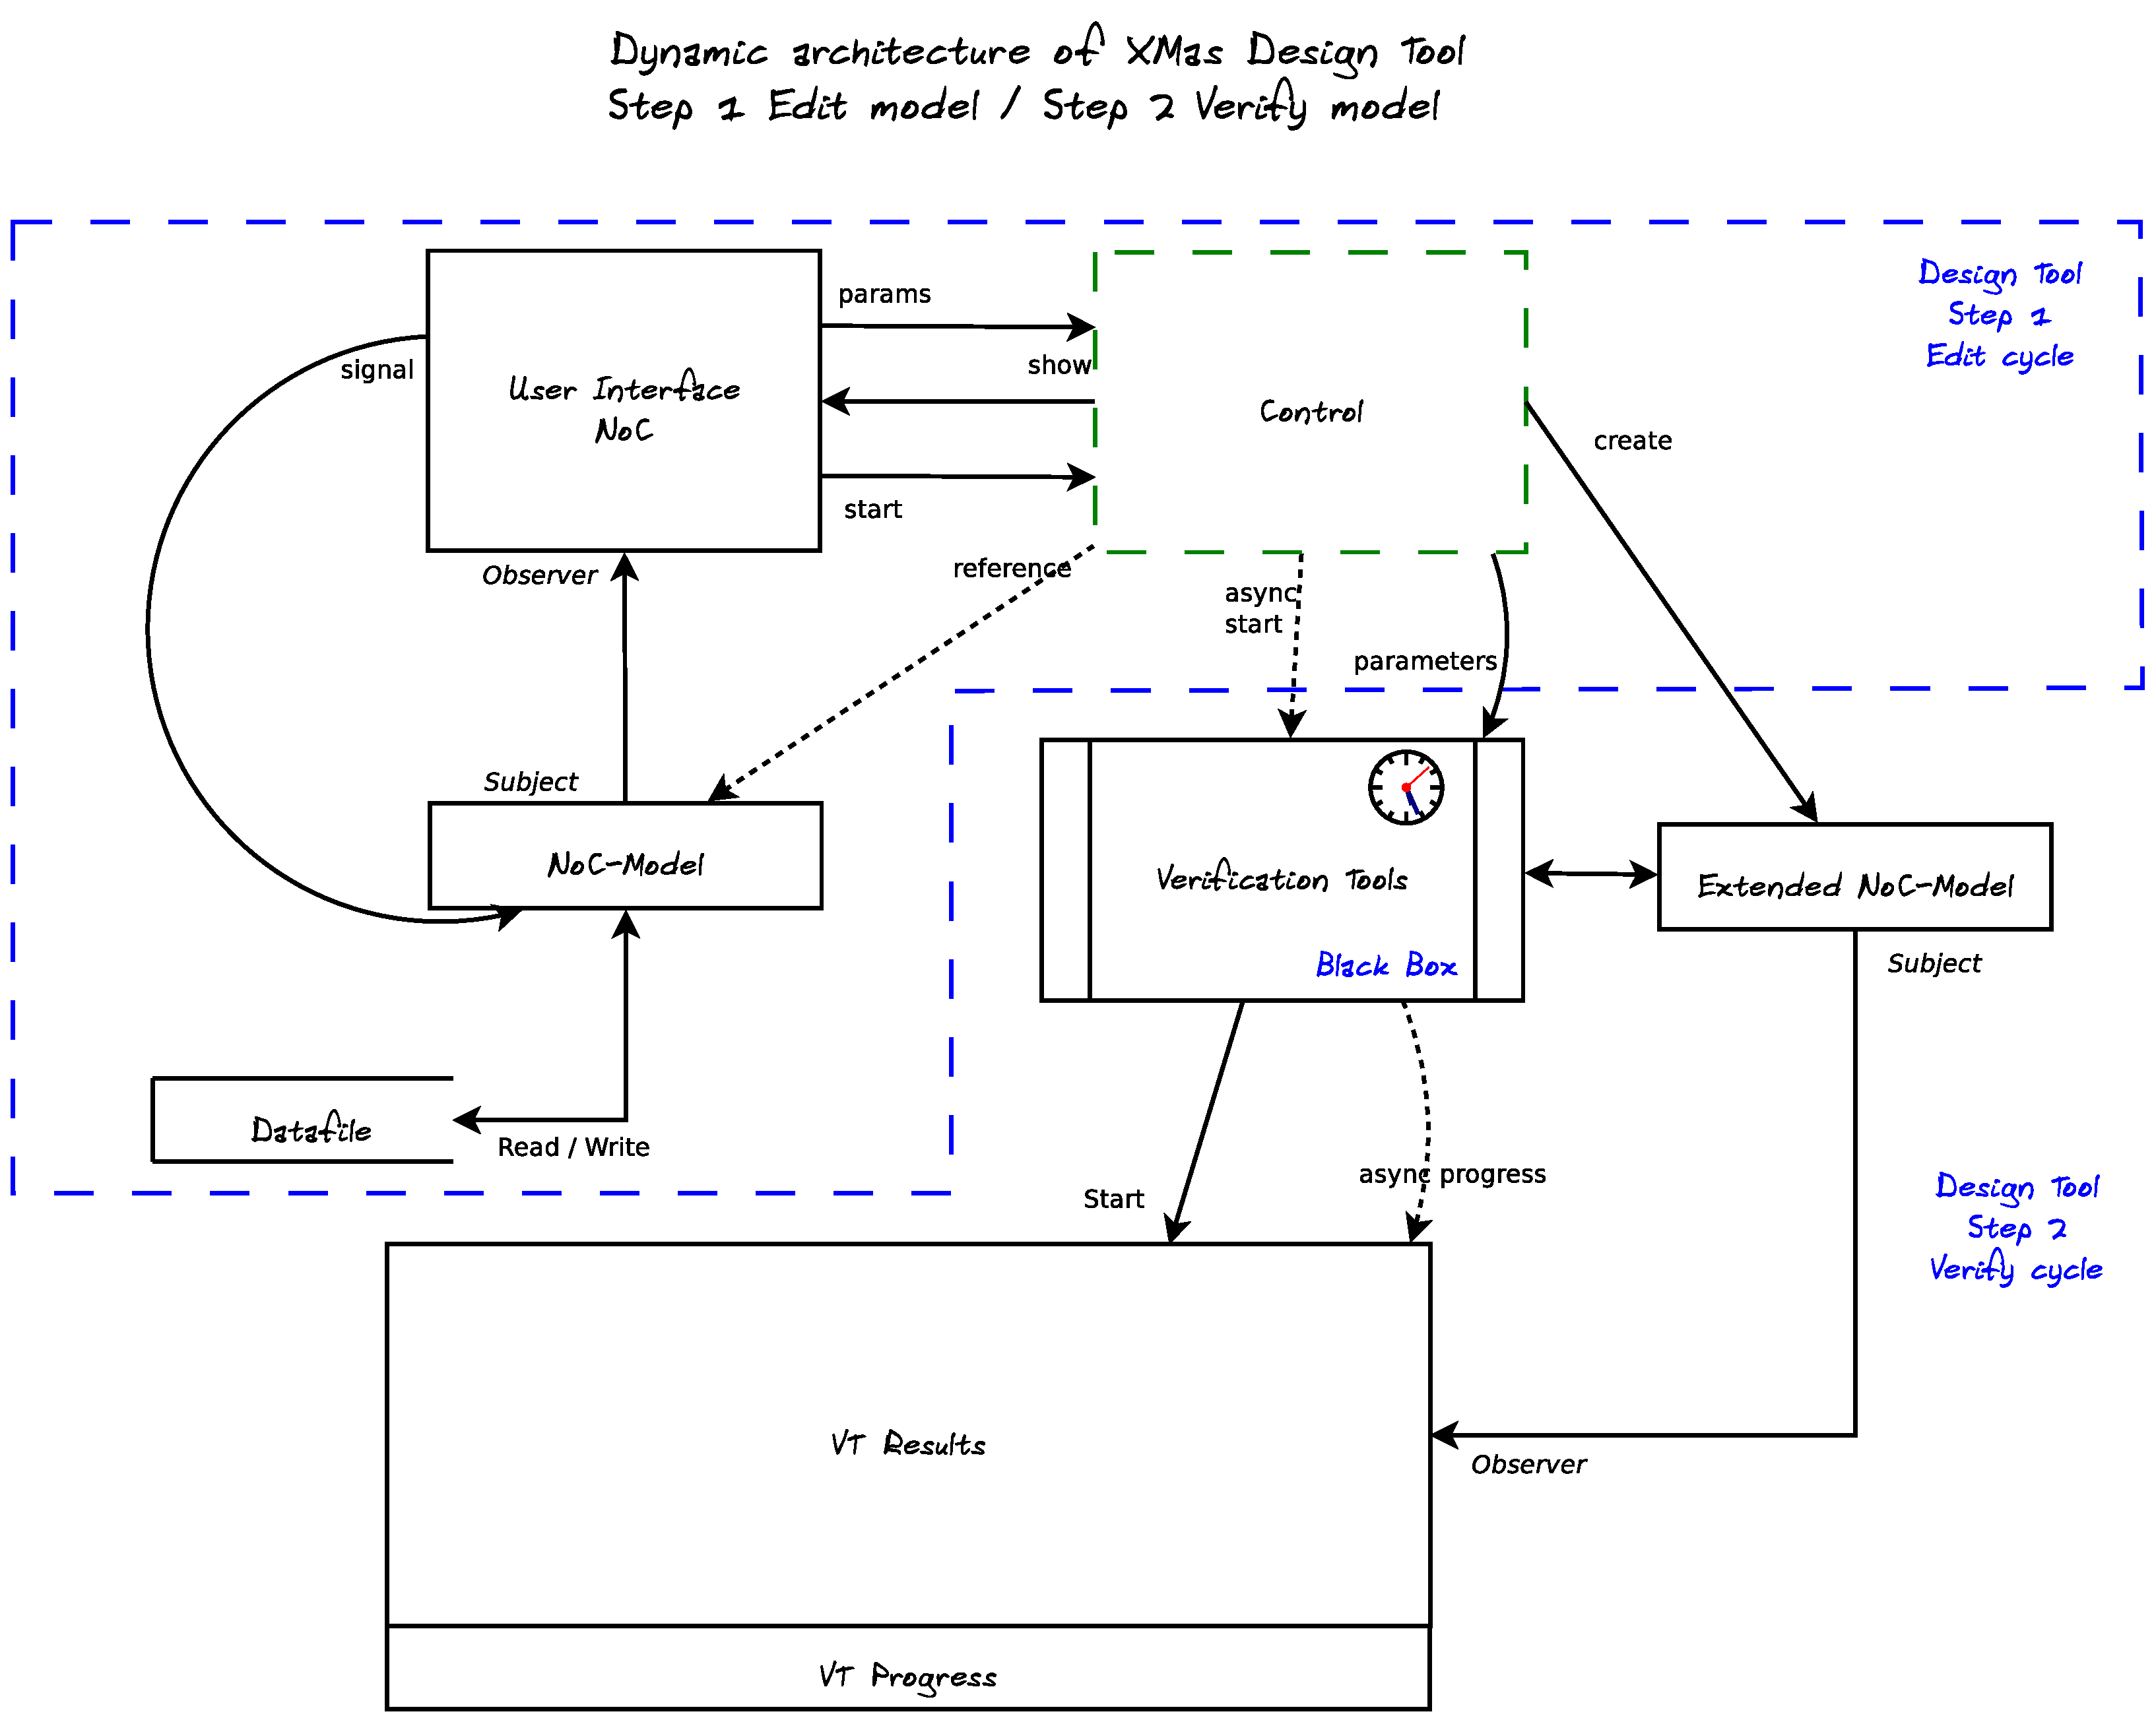
\includegraphics[width=.95\linewidth]{pictures/1c-architecture-dynamic-1}

\end{frame}

\begin{frame}{Implementation Data layer}

	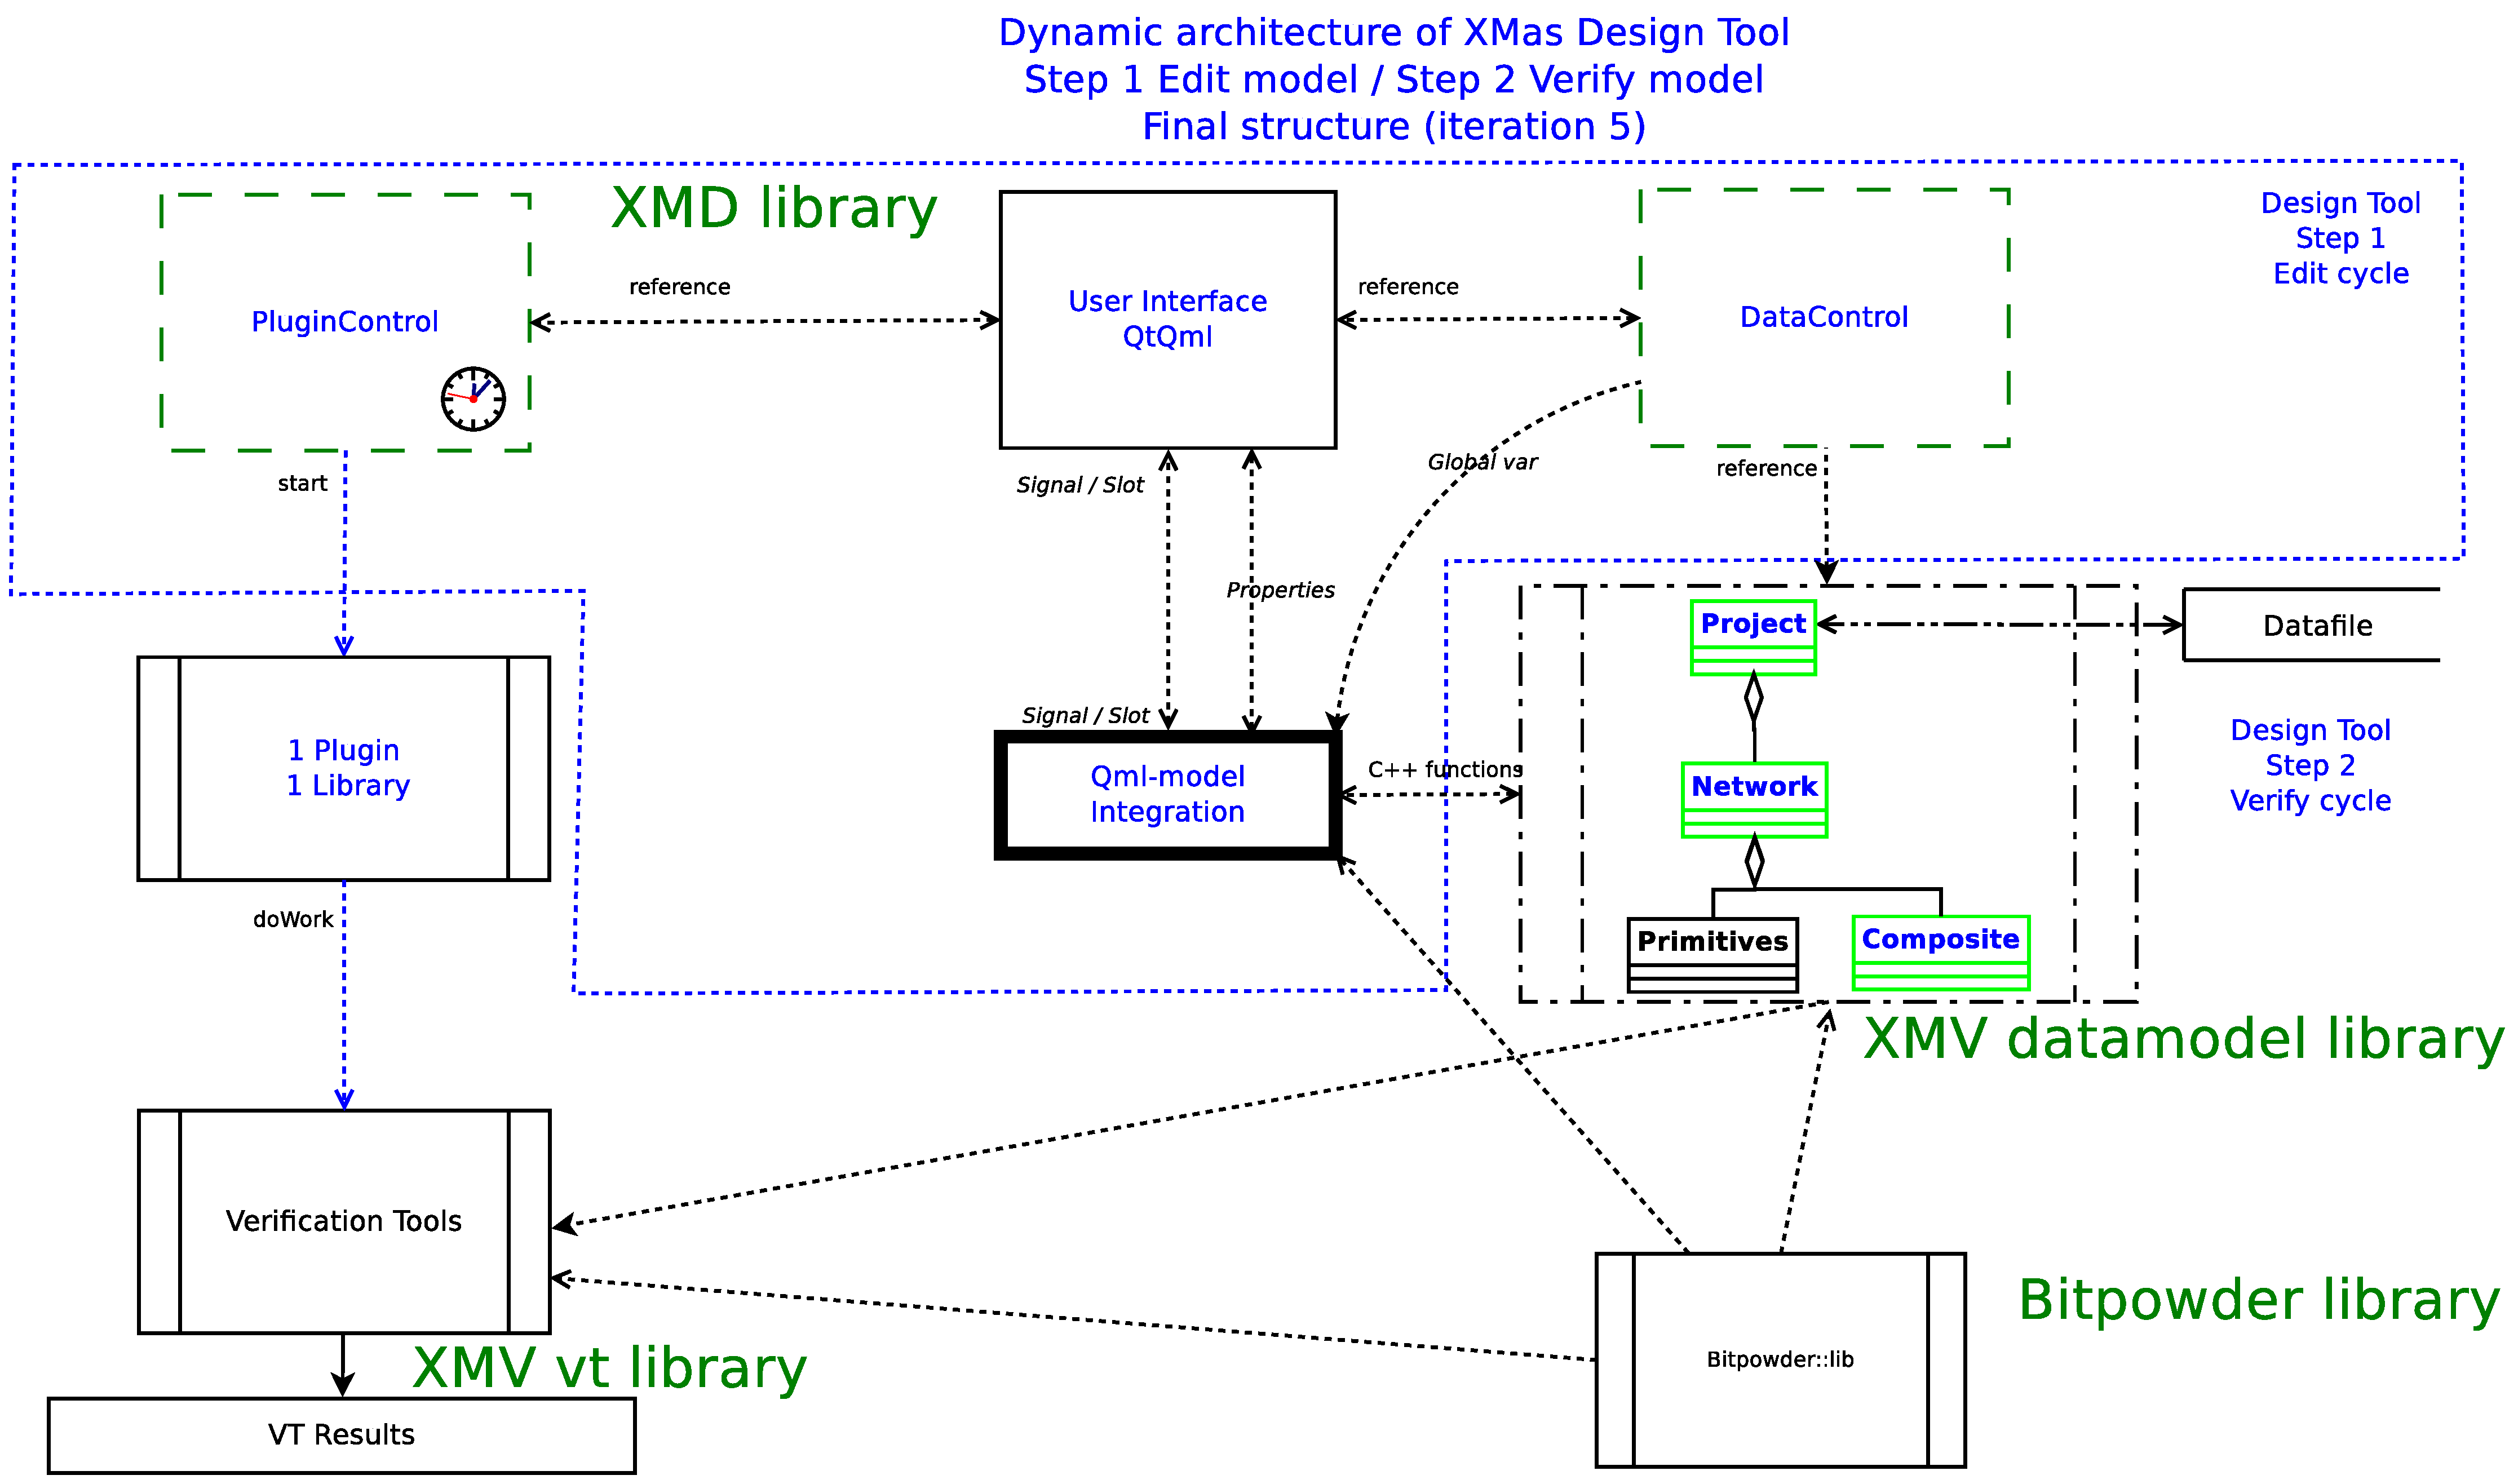
\includegraphics[width=.95\linewidth]{pictures/1c-architecture-dynamic-2}

\end{frame}

\begin{frame}{Project Reflection}
	\begin{itemize}
		\item {\bf Agile} 
				\begin{itemize}
					\item tools: skype: teamviewer, github, agilfant. Worked well.
					\item Internal communication: worked very well
					\item External communication: limited (OU reorg)
				\end{itemize}
		\item {\bf Planning}
				\begin{itemize}
					\item scheduling \& iterations: followed to a t.
					\item Influence OU reorg: risks increased
				\end{itemize}
		\item {\bf Design} 
			\begin{itemize}
				\item Switching to \qt				 (would do it again)
				\item Switching to \qml				 (might do it without tight xmas integration)
				\item Switching to tight xmas integration (underestimated consequences)
			\end{itemize}
	\end{itemize}
\end{frame}

\begin{frame}
	\begin{description}
		\item[Source code] github repo verwijzing
		\item[Documentation] github repo
	\end{description}
\end{frame}

\end{document}
